\documentclass[../../main.tex]{subfiles}

\begin{document}
Nachdem wir im letzten Abschnitt eine exakte Definition für Integrale durch das Aufsummieren von Rechtecken hergeleitet 
haben, wollen wir nun einen Weg finden, Integrale sinnvoll und exakt berechnen zu können, ohne Unmengen an Rechtecken
aufzusummieren.

Im Kapitel über Differentialrechnung hast du mit der Ableitung ein mächtiges Werkzeug zum Untersuchen von Funktionen
kennengelernt. Dieses Werkzeug verwenden wir nun auch, um Integrale zu berechnen, allerdings andersherum. 

Wenn wir eine Funktion, zum Beispiel $f(x)=x^2$, haben, können wir diese natürlich ableiten und bekommen dann $f'(x)=2x$. Wir können
aber auch in die andere Richtung gehen, uns also überlegen, welche Funktion wir ableiten müssen, damit wir $f(x)=x^2$ 
erhalten. Die Funktion, die wir dann suchen, heißt \textbf{Stammfunktion} von $f$. Mit ein bisschen Ausprobieren findest
du vielleicht eine Stammfunktion von $f(x)$, nämlich die Funktion $F(x)=\frac{1}{3}x^3$. Wenn du diese Funktion mit der
Potenzregel ableitest, erhältst du
\[F'(x)=\frac{1}{3}\cdot 3x^2=x^2=f(x).\]
Um die Stammfunktion von der ursprünglichen Definition zu unterscheiden, wird sie mit einem großen Buchstaben bezeichnet.
Deshalb haben wir sie $F(x)$ genannt.
\begin{definition}{Stammfunktion}
    Eine differenzierbare Funktion $F$ heißt \textbf{Stammfunktion} einer Funktion $f$, wenn  $F'=f$ gilt. 

    \emph{(Das heißt, die Stammfunktion einer Funktion $f$ ist eine Funktion, die man ableiten muss, um wieder $f$ zu erhalten.)}
\end{definition}
Wir werden später in diesem Abschnitt sehen, dass Stammfunktionen im engen Zusammenhang mit Integralen stehen. Wenn du
zu einer Funktion die Ableitung bestimmst, sagst du auch, dass du die Funktion ableitest. Wenn du stattdessen eine 
Stammfunktion bestimmst, sagt man dazu, dass du die Funktion \emph{integrierst}. Integrieren ist also genau das 
Gegenteil von Ableiten.
\begin{center}
    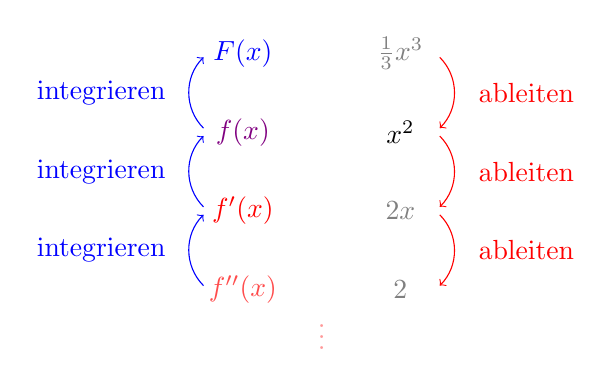
\begin{tikzpicture}
        \node[blue] at (0,1) {$F(x)$};
        \node[black!50!white] at (2,1) {$\frac{1}{3}x^3$};
        \node[violet] at (0,0) {$f(x)$};
        \node[black] at (2,0) {$x^2$};
        \node[red] at (0,-1) {$f'(x)$};
        \node[black!50!white] at (2,-1) {$2x$};
        \node[white!30!red] at (0,-2) {$f''(x)$};
        \node[black!50!white] at (2,-2) {$2$};
        \node[white!60!red] at (1,-2.5) {$\vdots$};
        \draw[blue,->] (-0.5,0.05) to[out=135, in=225] (-0.5,0.95);
        \draw[blue,->] (-0.5,-0.95) to[out=135, in=225] (-0.5,-0.05);
        \draw[blue,->] (-0.5,-1.95) to[out=135, in=225] (-0.5,-1.05);
        \draw[red,->] (2.5,-0.05) to[out=315, in=45] (2.5,-0.95);
        \draw[red,->] (2.5,-1.05) to[out=315, in=45] (2.5,-1.95);
        \draw[red,->] (2.5,0.95) to[out=315, in=45] (2.5,0.05);
        \node[blue] at (-1.8,0.5) {integrieren};
        \node[blue] at (-1.8,-0.5) {integrieren};
        \node[blue] at (-1.8,-1.5) {integrieren};
        \node[red] at (3.6,0.5) {ableiten};
        \node[red] at (3.6,-0.5) {ableiten};
        \node[red] at (3.6,-1.5) {ableiten};
    \end{tikzpicture}
\end{center}

\end{document}